\documentclass[12pt]{article}

\usepackage[margin=1in]{geometry}

\usepackage{amsmath, graphicx, caption, subcaption, xcolor}

\graphicspath{{res/}}

% I need a punchy title which is general enough
% to fit all three (if I can pull them off) points from the lab manual.
\title{\textcolor{red}{The Galactic Plane}}

\author{Lukas Finkbeiner}

\begin{document}

\maketitle

\begin{abstract}

We study

1. velocity patterns of various H clouds using Doppler shifts

2. black hole mass

3. accuracy of a spiral arm fit

results, uncertainties.

\end{abstract}

\section{Introduction and Background}

% However, I have not yet actually incorporated equation 8 into my analysis.
\begin{equation}
want two fit equations from the lab manual, eq.s 1 and 8
\end{equation}

We also want gain / calibration equations from lab 2.

Given certain patterns, how well does a spiral fit? We need to control for the total number of data. We want the normalization of any two compared sets to be the same (so, we scale accordingly). What numpy functions I used.

I definitely want to describe the Leuschner dish, some features in the signal chain, maybe just borrow the whole image and edit from there.

\section{Methods}

\quad \quad To observe the galactic plane, we have our trusty tracking script. After three labs' worth of development, it is almost correct!

We convert from galactic to topocentric coordinates using rotation matrices, as described in a previous report. How much should I include? If I describe the matrices again, that will certainly have to go in the introduction.

We probably want a basic run-down of a .fits file, but perhaps some of that can go in the introduction.

The Leuschner dish did not automatically report the frequency axis, \textcolor{red}{I think}. I should describe how I went from .fits file to calibrated spectrum (this includes determining the frequency axis).

%\begin{figure}
%	\centering
%	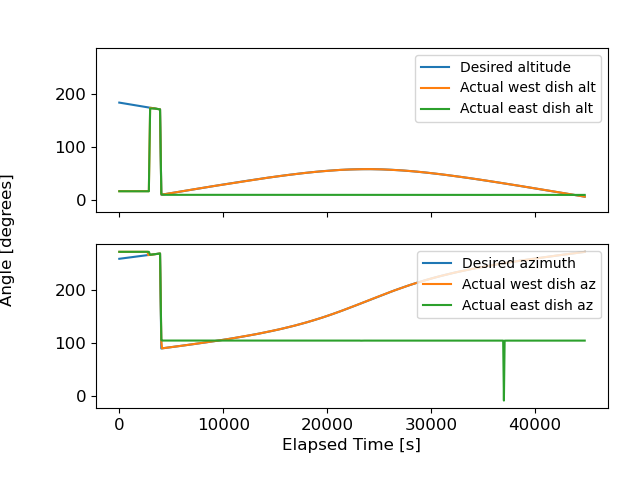
\includegraphics[width=.6\linewidth]{lockup}
%	\caption{These are the comparisons between the input dish angles (as computed with rotation matrices) and the true angles as reported by the dishes. The east dish displays little to no response, indicating that it was stuck for the virtually the entire capture.}
%	\label{fig:stuck}
%\end{figure}

\section{Observations}

\quad \quad What would be a good $introduction$ to the data? We have hundreds of raw spectra. I am not sure how to $succinctly$ describe observations before we get into the analysis.

\section{Analysis}

\quad \quad I should explain the process of taking a spectrum to a point on our galactic plane map (Doppler shift calculations, then orthographic projection). 

\section{Conclusions}

\quad \quad We seem to have at least a couple of results! How do I estimate the uncertainty on the Leuschner dish?

\section{Acknowledgments}

\quad \quad Who did what?

Theory and background provided by Aaron Parsons. ``LAB 4: Mapping the Galactic HI Line.'' Updated April 2020.

% Can we please get a bibliography this time?

\end{document}
